\documentclass[a4paper, 11pt]{article}
\usepackage[top=3cm, bottom=3cm, left=2.5cm, right=2.5cm]{geometry}
\usepackage{amsmath}
\usepackage{amsfonts}
\usepackage{graphicx}
\usepackage{psfrag}
\usepackage[utf8]{inputenc}
\usepackage[T1]{fontenc}
\usepackage[french]{babel}
\usepackage{hyperref}

\title{Rapport du Projet de Documents et Données Structurées \\M1 DSC : Analyse et Traitement de Factures}
\author{Pierre BONNEFOY, Ilyes ZEGHDALLOU,\\ Alexandre MARINE, Aloys LANA}


\begin{document}


\maketitle
\newpage
\tableofcontents

\newpage
\section{Définition du Projet}
Pour ce projet, nous avons choisit de nous lancer dans la création d'un logiciel d'analyse des Factures. Notre positionnement sera le suivant : nous sommes une entreprise tierce qui fournit un service à des clients (professionnels ou particuliers). Le client peut rentrer ses factures sur notre système et ensuite peut executer deux actions sur celle ci :
\begin{enumerate}
    \item Demander le montant total de toutes ses factures provenant d'une entreprise spécifique.
    \item Demander la liste des entreprises qui lui ont vendu un produit spécifique.
\end{enumerate}

\section{Modélisation de la Base de Données}
    \begin{center}
    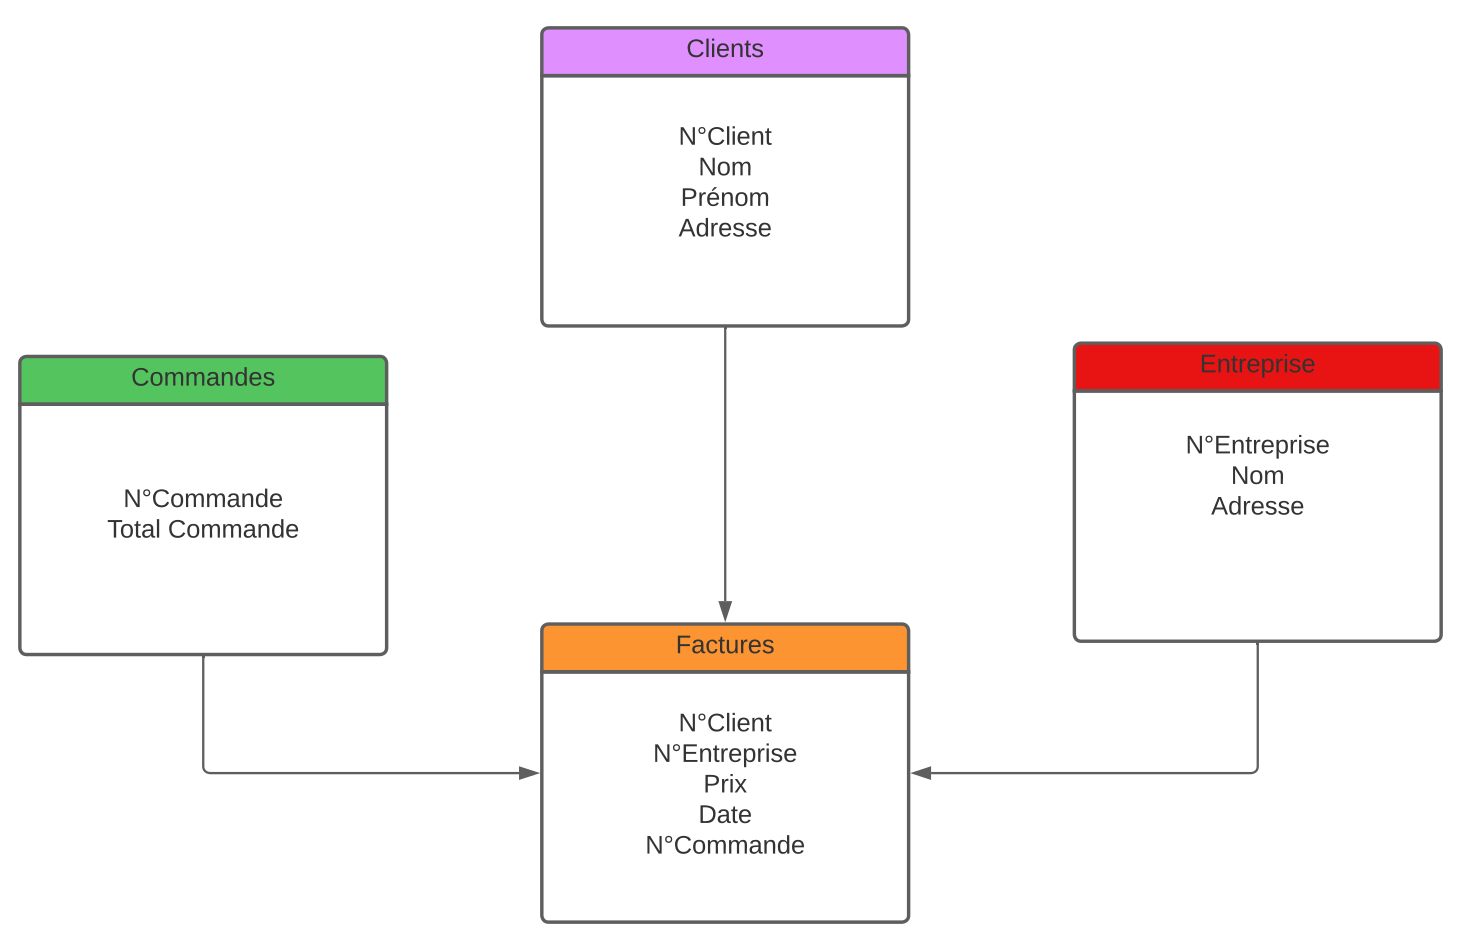
\includegraphics[scale=0.6]{schema_bdd.png}
    \end{center}

\section{Modélisations du Message 1}
    \subsection{Intitulé du Message}
        \subsubsection{Requête} 
        L'application métier demande à la Base de Données de lui envoyer le total de toutes les factures d'une entreprise cible.
        \subsubsection{Réponse}
        La Base de Données renvoie la somme de tous les totaux de chaque factures correspondant aux contraintes énoncées dans la requête.
    \subsection{Format JSON}
        \subsubsection{Requête}
        \begin{verbatim}
            {
            "requete": {
                "type": 1,
                "id_discussion": 1,
                "nom_client": "pierre",
                "num_siren": "123 152 152"
                }
            }
        \end{verbatim}
        
        \subsubsection{Réponse}
        \begin{verbatim}
            {
            "reponse" : {
                    "type" : 1,
                    "id_discussion" : 1,
                    "nom_client" : "Proton",
                    "total" : 21
                    }
            }
        \end{verbatim}
    \subsection{JSON Schema}
        \subsubsection{Requête}
        \begin{verbatim}
        {
        "requete": {
                type : "integer",
                id_discussion :"integer",
                nom_client : "string",
                num_siren :"string"
                }
        }

        \end{verbatim}
        
        \subsubsection{Réponse}
        \begin{verbatim}
        {
        "reponse": {
                type : "integer",
                id_discussion :"integer",
                nom_client : "string",
                total : "integer"
                }
        }
        \end{verbatim}
\section{Modélisations du Message 2}
    \subsection{Intitulé du Message}
        \subsubsection{Requête} 
        L'application métier demande à la Base de Données de lui envoyer la liste des entreprises lui ayant vendu un produit spécifique.
        \subsubsection{Réponse}
        La Base de Données renvoie la liste de toutes les entreprises lui ayant vendu ce produit.
    \subsection{Format JSON}
        \subsubsection{Requête}
        \begin{verbatim}
            {
            "requete": {
                "type": 2,
                "id_discussion": 1,
                "nom_client": "pierre",
                "nom_produit": "pommes"
                }
            }
        \end{verbatim}
            
        \subsubsection{Reponse}
        \begin{verbatim}
            {
            "reponse" : {
                        "type" : 2,
                        "id_discussion" : 1,
                        "nom_client" : "Proton",
                        "liste_entreprises" : ["giroud", "mbappe", "messi"]
                        }
            }
        \end{verbatim}
    \subsection{JSON Schema}
        \subsubsection{Requête}
        \begin{verbatim}
        {
        "requete": {
                type : "integer",
                id_discussion :"integer",
                nom_client : "string",
                nom_produit :"string"
                }
        }

        \end{verbatim}
        
        \subsubsection{Réponse}
        \begin{verbatim}
        {
        "reponse": {
                type : "integer",
                id_discussion :"integer",
                nom_client : "string",
                liste_entreprise : "[string]"
                }
        }
        \end{verbatim}

\section{Gestion de projet}
Pour ce projet, nous avons utilisé GitHub afin de stocker notre code source et d'avoir la possiblité d'accéder à notre code de manière facilitée. De plus, nous avons utilisé les tableaux de la partie Tâches et répartition afin de réalisé le suivi de nos tâches et de leurs état d'avancement;

\section{Tâches et répartition}
    \subsection{Analyse de Fichiers}
    \begin{center}
    \begin{tabular}{|c|c|c|c|}
        \hline
        Enoncé de la Tâche & Personne assignée & Etat & Priorité\\
        \hline
        \hline
        Determiner les informations à relevé  & Pierre BONNEFOY & Finit & HAUTE \\
        \hline
        Repérage des Mots-Clés & Pierre BONNEFOY & Finit & HAUTE  \\
        \hline
        Développer une procédure de relevé & Pierre BONNEFOY & Finit & HAUTE  \\
        \hline
        Adaptation à plusieurs types de factures & Pierre BONNEFOY & Finit & HAUTE  \\
        \hline
        Enregistrer dans la Base de Données & Pierre BONNEFOY & Finit & HAUTE  \\
        \hline
    \end{tabular}
    \end{center}

    \subsection{Communication de la Base de Données}
    \begin{center}
    \begin{tabular}{|c|c|c|c|}
        \hline
        Enoncé de la Tâche & Personne assignée & Etat & Priorité\\
        \hline
        \hline
        Créer une Base de Données  & Alexandre MARINE & Finit & HAUTE \\
        \hline
        Gérer l'accés a la Base de Données  & Alexandre MARINE & Finit & HAUTE \\
        \hline
        Réception des requête de AM  & Alexandre MARINE & Finit & HAUTE \\
        \hline
        Générer la réponse en JSON  & Alexandre MARINE & Finit & HAUTE \\
        \hline
    \end{tabular}
    \end{center}

    \subsection{Génération des requêtes depuis l'application métier}
    \begin{center}
    \begin{tabular}{|c|c|c|c|}
        \hline
        Enoncé de la Tâche & Personne assignée & Etat & Priorité\\
        \hline
        \hline
        Creer le formulaire du message 1  & Ilyes ZEGHDALLOU & Finit & HAUTE \\
        \hline
        Creer le formulaire du message 2  & Ilyes ZEGHDALLOU & Finit & HAUTE \\
        \hline
        Génération du fichier JSON de la requête  & Ilyes ZEGHDALLOU & Finit & HAUTE \\
        \hline
    \end{tabular}
    \end{center}

    \subsection{Réception des Réponses et Affichage coté Application Métier}
    \begin{center}
    \begin{tabular}{|c|c|c|c|}
        \hline
        Enoncé de la Tâche & Personne assignée & Etat & Priorité\\
        \hline
        \hline
        Scruter le Dossier de Simulation du réseau  & Aloys LANA & Finit & HAUTE \\
        \hline
        Récuperer les données du fichier JSON  & Aloys LANA & Finit & HAUTE \\
        \hline
        Afficher les résultats  & Aloys LANA & Finit & HAUTE \\
        \hline
        Supprimer les anciens messages  & Aloys LANA & Finit & HAUTE \\
        \hline
    \end{tabular}
    \end{center}

\section{Choix des technologies}
    Pour ce projet, nous avons choisit d'utiliser le langage Python au vu de sa simplicité d'utilisation et de sa diversité de bibliothèques permettant de nous facilité le travail.\\
    En voici la liste :
    \begin{enumerate}
        \item json : une bibliothèque permettant de traiter et de générer des fichiers JSON.
        \item tkinter : une bibliothèque graphique qui nous a permit de réalisé l'interface utilisateur.
        \item mysql-connector : Afin de réaliser les requêtes pour remplir la Base de Données et récupérer les informations nécéssaires à la réponse de cette dernière.
        \item watchdog : Afin de pouvoir faire un observer afin de simuler le réseau dans un dossier.
    \end{enumerate}


\section{Problèmes Rencontrés}
    \subsection{Analyse des documents}
    Nous avons eu de nombreux problèmes au niveau de l'analyse :
    \begin{enumerate}
        \item Nous avions initialement décidé d'utilisé l'adresse email comme identifiant client. Cela a rapidement à rapidement montrer ses limites. En effet, il arrivait que notre programme confondent l'adresse email du client avec celle du vendeur. De plus, l'adresse email ne semble pas être une donnée impérative dans les factures. Contrairement à elle, le nom et adresse des entreprises elles le sont.
        \item La détermination des mots clés utiles au relevé d'informations.
    \end{enumerate}

    \subsection{Base de Données}
    Concernant les problèmes liés à la Base de Données :
    \begin{enumerate}
        \item Suite au problème de l'analyseur dont nous avons du modifier les informations relevées. Nous avons dû faire une refonte de notre modélisation.
        \item Les variables entières et les chaînes étant immuables, il nous a fallu outre-passé la restricition de l'interface graphique pas l'utilisation de l'objet liste. Cela empéché les return des fonctions.
        \item Idem concernant la récupération des infos en provenance du système de requêtes.
        \item Mise en place d'un Watcher sous forme de Thread afin de d'évité que cela ne bloque l'interface graphique.
        \item Problème de formatage dans les requêtes SQL.
    \end{enumerate}

    \subsection{Application Métier}
    Initialement, nous avions décidé d'utilisé les technologies Web (HTML, CSS et JS) afin de réalisé l'application métier. Cela a posé de nombreux problèmes nottament la lecture de fichiers locaux et leur création. Nous avons donc décidé de basculer sur Python qui nous a largement aidé à régler ce problème.
    De plus, nous avons eu un léger problèmes afin de communiquer avec la Base de Données. En effet, Aloys et Ilyes travaillant sous Windows et Alexandre sous Linux, les deux systèmes ne géraient pas de manière similaire les chemins et les Créations et Modifications de fichier. Nous avons donc du travailler avec Alexandre afin de corriger ce problème.

\section{Bilan du projet}
Nous sommes assez satisfaits du résultat de notre projet. En effet, notre application permet d'analyser 3 types de factures différents. La communication entre l'Application Métier et la Base de Données est fonctionnelle et fluide.
Nous avons pu consacrer du temps à la réalisation d'interface graphique abouties.

\section{Conclusion}
Pour conclure, ce projet nous a permis de nous familiariser avec le format JSON, qui pour la majorité d'entre nous n'avais jamais été manipuler. Nous avons eu l'occasion de manipuler TKinter afin de réalisé des Interfaces Graphiques en Python, ainsi que WatchDog pour gérer les fichiers systèmes. Il nous a aussi fournit une approche de travail qui se rapproche de celle d'une entreprise (communication, documentation, ...). 

\end{document}

